\section{はじめに}
屋内位置推定技術は,現代社会において重要な役割を果たしており様々な活用が期待できる.
屋内位置推定技術が使用される一例として,ショッピングモール施設内でのナビゲーションシステムが挙げられる.
\footnote{https://www.kkc.co.jp/service/blog/\\indoor-outdoor-positioning/achievement/article/9725/}
このシステムでは顧客の位置情報を元にして,現在地周辺にある店舗のおすすめ情報や目的地までのナビゲーションを提供する.
屋外における位置推定技術としてGPSが広く利用されているが,屋内環境では建物の壁や天井がGPS衛星からの電波を遮断してしまい,位置推定精度が大きく低下してしまう問題がある.
そのため別のアプローチが必要とされている.

屋内位置推定の手法には絶対位置推定手法,相対位置推定手法がある.
絶対位置推定手法は経度や緯度などの特定の基準点を元に位置を推定する手法である.
その代表例としてはWi-Fi,BLE,地磁気などの情報を利用したものがある.
Wi-FiやBLEなどを電波を利用した屋内位置推定は,アクセスポイントからの信号強度を利用して位置推定を行う.
予めアクセスポイントの基地局情報が判明している場合,3つのアクセスポイントからの電波強度を利用して三角測量を行う手法がある.
相対位置推定手法はある特定の基準点からの相対的な位置を推定する手法である.
その代表例としてPDR(Pedestian Dead Reckoning)がある.
PDRは,加速度計,ジャイロスコープ,などのセンサを利用して歩行者の歩幅,進行方向,ステップタイミングを推定する.
その情報を元に歩行者の移動を累積的に計算し,基準位置からの相対的な位置を推定する手法である.

ハイブリット位置推定手法はPDRと絶対位置推定を組み合わた手法である.
絶対位置推定は特定の環境に依存しており,その環境がない場所では推定できない問題点がある.
PDRによる推定には初期位置の初期進行方向の情報が必ず必要な問題がある.
またPDRではセンサーのわずかな誤差が累積されため,長時間に及ぶ歩行では軌跡の形状が大きく変化してしまう問題がある.
ハイブリット手法では両方の手法を組み合わせてこれらの問題の解決を行う.
この手法は屋内位置推定の手法の中で有用な手法として様々な情報を用いた推定手法が研究がされている.

しかしこれらの研究は特定の条件下でのPDRと組み合わせたものが多く,他の条件下では推定が難しい.
例としてWi-Fiを利用した方法の場合,基地局の位置が事前に把握できているケースとできないケースが考えられる.
また追加で補正に利用できる条件がある場合も考えられる.
環境によって補正に使用できる情報は変化する.
多くの環境での使用を想定したような屋内位置推定ライブラリは存在しない

本研究では様々な環境と状況に対応できるPDRベースの屋内位置推定ライブラリの基礎検討を行う.
本研究の概要を\ref{fig:overview}に示す.
推定に使用できる情報をセンサ情報と環境情報に分け,これらの情報を元にPDRとその補正を行うライブラリを構築し提供する.
これらの関数はそれぞれの環境や条件に応じて使用でき組合せて使えるような形を目指す.

\begin{figure}[h]
	\centering
	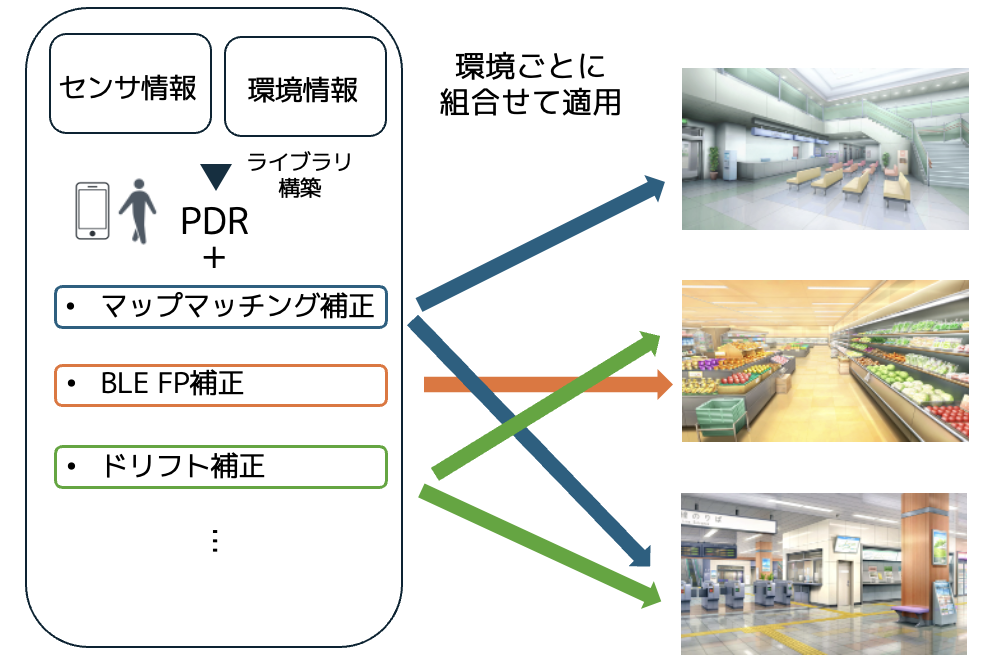
\includegraphics[width=80mm]{image/first.png}
	\caption{様々な状況と環境に対応できる\\PDRベースの
		屋内位置推定ライブラリの概要}    \label{fig:overview}
\end{figure}
